%-----------------------------------------------------------------------------%
\chapter{\babEmpat}
\label{bab:4}

Bab ini menjelaskan detail arsitektur dan implementasinya. Perbedaan dari performa aplikasi ini memberikan kesempatan untuk melakukan optimisasi desain sistem terdistribusi ke depannya. Detail parameter dan cara melakukan tolok ukur performa terhadap variasi aplikasi PeerToCP juga akan dipaparkan lebih lanjut dalam bab ini pada subbab~\ref{sec:desain_evaluasi} tentang desain dan parameter evaluasi. Bab ini juga akan memberikan penjelasan singkat serta alasan pemilihan beberapa teknologi, termasuk \textit{library} dan \textit{modul} yang digunakan dalam implementasi aplikasi PeerToCP. Sebagai konteks, bagian awal dari bab ini menjelaskan mengenai teknologi yang digunakan untuk implementasi, diikuti dengan desain sistem serta detail sudut pandang pengguna terhadap \textit{usecase} aplikasi.

\section{\textit{Library} dan \textit{Framework} Terkait}

Terdapat beberapa aplikasi dan \textit{library} yang terkait dalam pengembangan sistem aplikasi PeerToCP yang dibahas dalam penelitian ini. Berbagai \textit{framework}, \textit{library}, dan sistem modul ini merupakan hasil penelitian oleh para pengembang sebelumnya. Pemilihan penggunaan untuk setiap teknologi ini dipertimbangkan dengan alasan tertentu, salah satunya adalah Electron, yang menjadi basis pengembangan aplikasi \textit{desktop}.

Electron merupakan salah satu \textit{framework} aplikasi \textit{desktop} yang melibatkan HTML, CSS, dan JavaScript. Bagian belakang atau \textit{backend} dari Electron berjalan dengan lingkungan \textit{runtime} Node.js~\citep{kredpattanakul2018transforming, miglanielectron}. Node.js merupakan bahasa yang menggunakan \textit{syntax} yang serupa dengan Javascript dan dapat dikompilasi melalui kompilator yang disebut V8 engine~\citep{tilkov2010node}. Bagian tampilan atau \textit{frontend} dari Electron memanfaatkan aplikasi \textit{Chromium} yang dapat mengolah bahasa \textit{markup} web, seperti HTML (\textit{HyperText Markup Language}), CSS (\textit{Cascading Style Sheets}), serta JavaScript.

Salah satu keuntungan menggunakan Electron adalah aplikasinya yang bersifat \textit{cross-platform} atau dapat berjalan di beragam sistem operasi, seperti Windows, GNU/Linux, atau MacOS. Keuntungan lainnya ialah karena bersifat aplikasi desktop, Electron dapat mengakses berbagai macam fungsi antar muka sistem operasi, seperti memanggil subproses pada sistem dan menulis berkas. Karena \textit{frontend}-nya yang menggunakan bahasa web pula, aplikasi yang dibuat dengan Electron cenderung lebih mudah untuk dipindahkan dan diadaptasi dengan fungsi terbatas pada web. Selain \textit{Electron}, masih terdapat beberapa alternatif \textit{desktop-based framework} lain seperti Qt yang berbasis C++ dan Tauri yang berbasis Rust. Pemilihan Electron dipilih karena beberapa \textit{library} \textit{operational transformation}, \textit{CRDT}, \textit{WebSocket}, dan \textit{WebRTC} yang umum digunakan sudah tersedia implementasinya dalam JavaScript dan dapat digunakan melalui Node.js.

Untuk memenuhi kebutuhan komponen editor kode sebagai media interaksi pengguna dengan sistem pada \textit{frontend}, digunakan \textit{Codemirror}. Codemirror merupakan komponen \textit{frontend} editor kode yang dapat diolah oleh peramban web. Codemirror menyediakan banyak ekstensi, aksesibilitas tinggi, serta dukungan untuk berbagai macam bahasa pemrograman. Codemirror berguna untuk menampilkan editor kode dan memiliki ekstensi yang menghubungkannya dengan Yjs, sebuah library CRDT dan sudah diuji oleh pengembang Codemirror.

Yjs sendiri merupakan sebuah \textit{framework library} yang mengimplementasi CRDT yang disebut dengan YATA (\textit{Yet Another Transformation Approach})~\citep{Nicolaescu2016yjs}. Yjs terdiri dari beberapa bagian, yaitu YDocs yang merupakan bagian utama implementasi berbagai struktur data untuk CRDT. Dalam penelitian ini, digunakan tiga struktur data CRDT yang abstraksinya berbeda. YText merupakan variasi CRDT untuk operasi-operasi pada \textit{text editor}, serta YMap dan YArray yang dikombinasikan untuk menyimpan \textit{shell} dan riwayatnya. Yjs sendiri merupakan \textit{library} yang tidak terpaku pada sebuah arsitektur. Terdapat dua \textit{provider} jaringan yang dapat berintegrasi dengan YDocs, yaitu YWebRTC dan YWebSocket. Kedua provider ini masing-masing mengintegrasikannya dengan jaringan \textit{full-mesh peer-to-peer} dan \textit{client-server} secara berturut-turut. Yjs memiliki banyak pengembang aktif dari komunitas dan hingga kini masih di-\textit{maintain} dan dikembangkan, sehingga \textit{library} ini dipilih untuk penelitian ini.

Untuk variasi \textit{operational transformation} dari PeerToCP, penelitian ini memanfaatkan ekstensi \textit{collaborative editing} dari CodeMirror yaitu @codemirror/collab. \textit{Provider} jaringan untuk arsitektur \textit{client-server} yang dikembangkan untuk metode \textit{operational transformation} ini pula menggunakan \textit{library} rpc-websockets yang dimodifikasi sehingga dapat dimanfaatkan untuk melakukan \textit{broadcast}, \textit{specific-messaging} ke klien tertentu, serta fungsionalitas pemanggilan RPC (\textit{Remote-Procedure Call}) berbentuk \textit{promise} secara \textit{asynchronous} dan \textit{non-blocking}.

Pada variasi PeerToCP dengan metode OT, penyimpanan \textit{shell} diimplementasi tanpa OT untuk menyederhanakan kompleksitas program. Data \textit{shell} dapat disimpan menggunakan \textit{array} yang bersifat \textit{grow-only}. Operasi-operasi yang dapat dilakukan pada \textit{shell} program berjalan merupakan \textit{keystroke} masukan klien. Secara khusus, beberapa \textit{keystroke} di-\textit{treat} oleh terminal secara literal dan program sendiri lah yang harus menangani bagaimana \textit{keystroke} tersebut akan diperlakukan. Misalnya, operasi penghapusan atau melakukan \textit{backspace} secara bawaan pada masukan \textit{shell} diartikan sebagai menambahkan tiga karakter ``$\texttt{\char`\\ b \char`\\ b}$'' (tanpa tanda petik) atau ekuivalen dengan memindahkan \textit{cursor} ke kiri, memasukkan karakter \textit{whitespace}, dan memindahkan \textit{cursor} ke kiri lagi tanpa menghapus karakter secara harfiah. Dalam penelitian ini, aspek kolaborasi dari \textit{shell} memperlakukan setiap klien untuk memberikan \textit{keystroke} pada satu kanal yang sama tanpa \textit{positional cursor} ganda seperti pada editor kode.

Untuk memenuhi komponen penjalanan program yang dapat diakses oleh setiap klien dalam jaringan, dibutuhkan suatu \textit{library} untuk mengakses sistem operasi untuk melakukan kompilasi terhadap kode. Kompilasi merupakan proses mengonversi kode dari bahasa dengan level yang lebih tinggi dan dapat dimengerti oleh manusia menjadi kode biner yang dapat dimengerti oleh mesin~\citep{aho1985compilers}. Pada penelitian ini, selain editor kode yang bersifat kolaboratif, proses kompilasi kode tunggal juga hendaknya dapat dilakukan oleh salah satu pengguna. Proses kompilasi ini membutuhkan kompilator yang terpasang pada suatu sistem operasi. Pada Node.js, salah satu \textit{library} yang dapat digunakan untuk mengaksesnya ialah Node-pty.

Node-pty merupakan \textit{library} Node.js yang memberikan antarmuka untuk melakukan \textit{fork} proses dengan deskriptor berkas \textit{pseudoterminal}. Node-pty mengizinkan adanya aliran data untuk baca dan tulis dengan proses berjalan pada kernel. Node-pty berguna untuk menjalankan berkas hasil kompilasi yang bersifat CLI (\textit{Command Line Interface}) yang tidak memiliki tampilan grafik untuk pengguna. Node-pty dipilih karena banyak digunakan dan bersifat \textit{cross-platform} mendukung sistem operasi Windows, GNU/Linux, dan MacOS. Aplikasi ini juga membutuhkan bagian \textit{frontend} untuk menampilkannya, dan digunakan Xterm.js. \textit{Library} ini merupakan salah satu komponen yang menampilkan terminal melalui bahasa yang dapat diolah oleh web. Xterm.js memiliki antarmuka yang bisa menerima dan meneruskan data dari peramban (\textit{browser}) yang dapat dihubungkan dengan sebuah proses berjalan pada sistem. Xterm.js dikembangkan tanpa memerlukan dependensi, sehingga dipilih dalam pengembangan sistem ini.

\section{Desain Sistem}

Aplikasi PeerToCP didesain sebagai sebuah aplikasi \textit{desktop-based}, yang berarti dijalankan tidak melalui browser \textit{web}. Pilihan ini dikonsiderasi karena untuk mempermudah akses secara \textit{offline}, sehingga tidak dibutuhkan koneksi internet untuk mengakses aplikasi. Selain itu, fitur kompilasi pada suatu \textit{peer} memerlukan akses \textit{system-call} yang tidak disediakan pada API web-browser~\citep{v8, spidermonkey}. Hal ini ditetapkan agar \textit{script} yang dijalankan pada mesin browser tidak dapat menyerang komputer secara langsung. Berikut ialah \textit{diagram activity} yang menunjukkan garis besar penggunaan aplikasi.

\begin{figure}
    \centering
    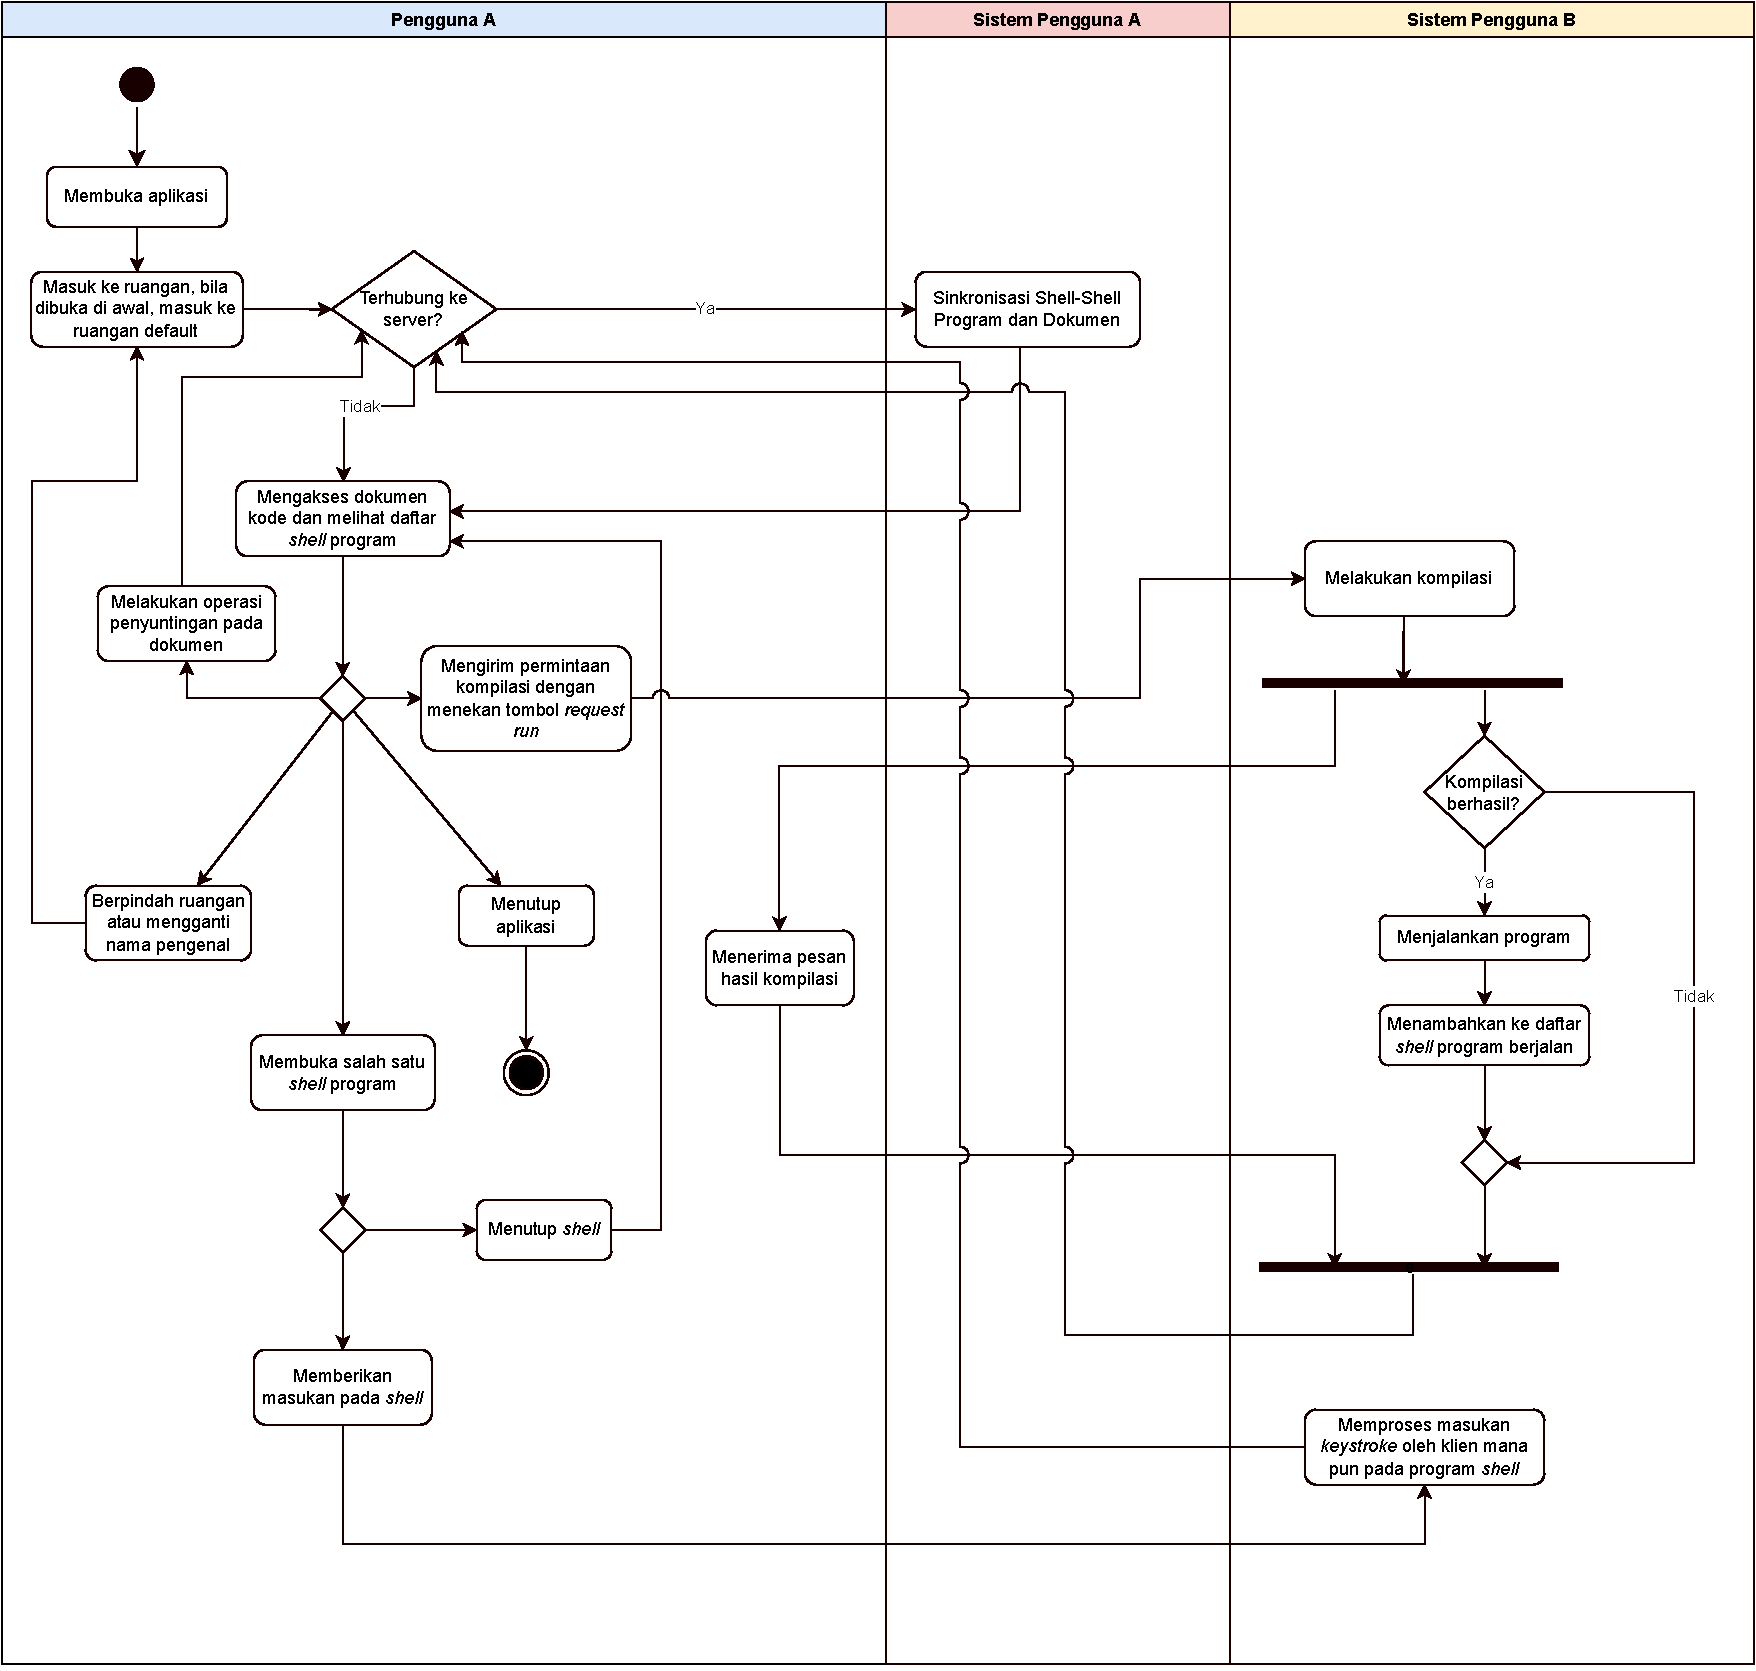
\includegraphics[scale=0.5]{assets/skripsi/Activity_Diagram}
    \caption{\textit{Activity Diagram} Alur Penggunaan Secara \textit{High Level}}
    \label{fig:activity}
\end{figure}

Saat pengguna membuka aplikasi, pengguna akan diarahkan untuk masuk ke ruangan awal secara \textit{default}. Pengguna dapat melakukan operasi-operasi penyuntingan pada dokumen dan sinkronisasi dilakukan secara terus-menerus dengan \textit{publish-subscribe design pattern} sehingga memberikan respons tanpa perlu mengecek atau \textit{polling} secara terus menerus saat terjadi \textit{update} yang terjadi antarklien. \textit{Request} atau permintaan kompilasi dapat diajukan kepada klien mana pun pada jaringan, termasuk permintaan untuk klien ini sendiri. Aplikasi PeerToCP akan mencoba mengirimkan pesan kepada klien yang ditentukan tanpa mengabari tanpa intervesi dari klien lain dalam jaringan. Apabila permintaan berhasil diterima, sistem pada klien yang diminta akan melakukan proses kompilasi dan memasukkan \textit{shell} program berjalan dengan ID tertentu ke daftar \textit{shell} yang dapat diakses ke setiap klien dalam jaringan. Daftar \textit{shell} dan kontennya ini disimpan dalam bentuk \textit{object} pada \textit{JavaScript}.

Pada Gambar~\ref{fig:activity}, perilaku sinkronisasi \textit{shell-shell} program dan dokumen dilakukan tergantung dengan variasi implementasi dari program. Pada arsitektur \textit{client-server}, sistem aplikasi pengguna A akan berhubungan dan melakukan sinkronisasi dengan server. Sementara pada arsitektur \textit{peer-to-peer}, sistem aplikasi pengguna A akan berhubungan langsung dan melakukan sinkronisasi dengan \textit{peer} atau klien lain. Selain itu, permintaan dan transmisi pesan hasil kompilasi dilakukan melalui pengiriman pesan secara langsung pada arsitektur \textit{peer-to-peer}, namun harus melalui perantara server pada arsitektur \textit{client-server}. Detail implementasi dan arsitektur detail aplikasi akan dirincikan pada Subbab~\ref{sec:desain_crdt} dan ~\ref{sec:design_ot}

\section{CRDT (\textit{Conflict-Free Replicated Data Type}) Berbasis \textit{Peer-To-Peer} dan \textit{Client-Server}}
\label{sec:desain_crdt}

\begin{figure}
    \centering
    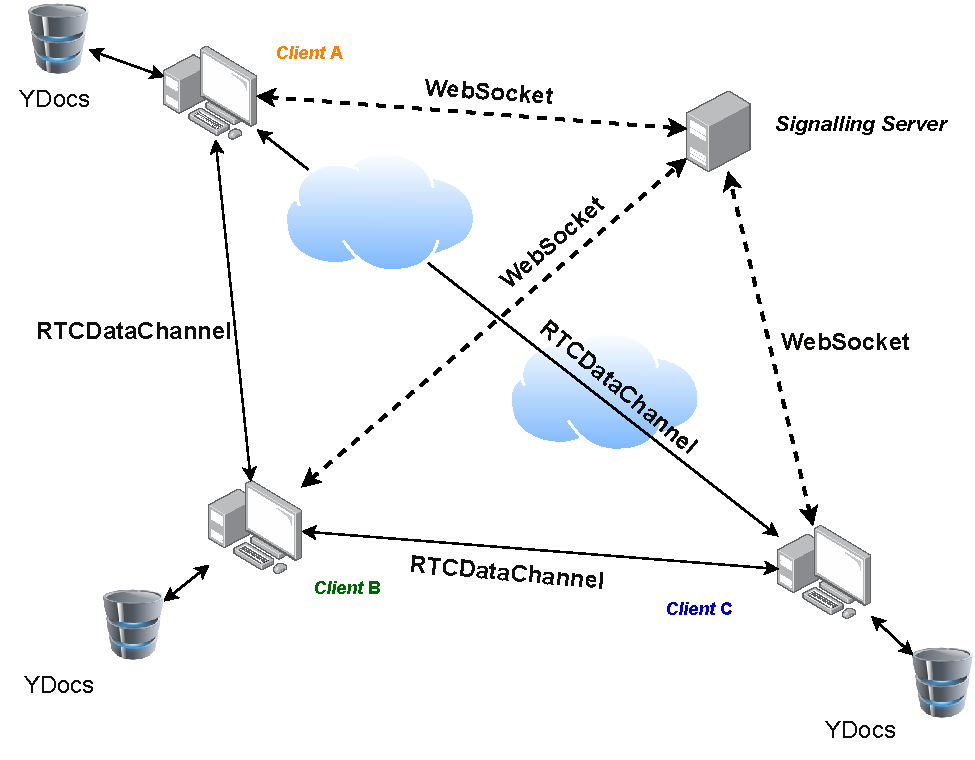
\includegraphics[scale=0.65]{assets/skripsi/Arsitektur_WebRTC_CRDT}
    \caption{Arsitektur yang Menggunakan WebRTC dengan \textit{WebSocket Signalling} dan CRDT}
\end{figure}

CRDT pada dua skenario arsitektur dalam penelitian ini menggunakan library CRDT Yjs yang menggunakan algoritma YATA~\citep{Nicolaescu2016yjs} yang dijelaskan pada subbab~\ref{sec:penelitian_terkait}. Setiap \textit{peer} atau klien memiliki replika besar yang direpresentasikan dalam tipe data YDocs. YDocs dapat terdiri dari beberapa CRDT untuk menyimpan data-data yang akan dijaga di setiap \textit{peer} atau klien. Implementasi dari variasi \textit{peer-to-peer} menggunakan \textit{library} penyedia jaringan YWebRTC yang telah dimodifikasi untuk memiliki antarmuka untuk mengirim pesan ke \textit{peer} tertentu melalui jaringan RTCDataChannel. Bagian \textit{shell} pada aplikasi direpresentasikan sebagai sebuah CRDT \textit{map} yang memetakan ID ke sebuah CRDT \textit{grow-only array} yang merepresentasikan \textit{shell} yang berjalan pada salah satu \textit{peer host}. \textit{Keystroke} yang diberikan oleh sebuah \textit{peer} tertentu akan dikirim langsung pada \textit{peer host} yang menjalankannya, kemudian \textit{peer host} akan menambahkan hasil \textit{keystroke} pada CRDT-nya.

\begin{figure}
    \centering
    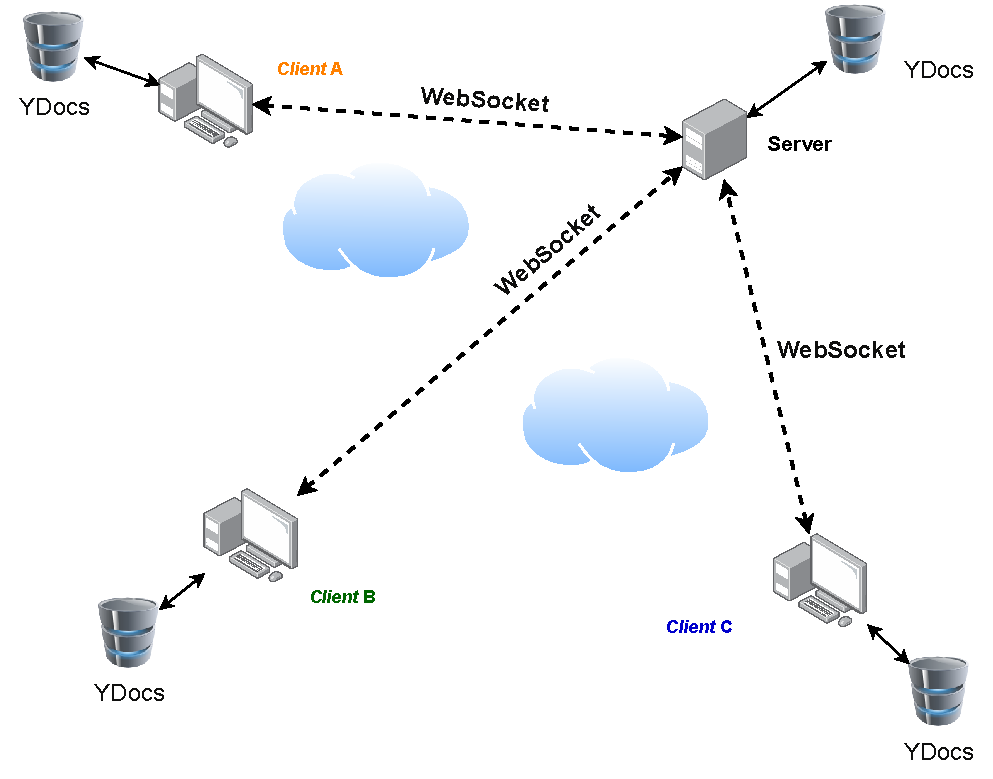
\includegraphics[scale=0.65]{assets/skripsi/Arsitektur_WebSocket_CRDT}
    \caption{Arsitektur yang Menggunakan WebSocket dan \textit{CRDT}}
\end{figure}

Perbedaan antara kedua implementasi arsitektur CRDT ini terdapat pada \textit{provider} atau penyedia jaringannya. Pada arsitektur \textit{client-server}, penelitian ini menggunakan \textit{library} YWebSocket yang telah dimodifikasi pula untuk dapat mengirim pesan kepada klien lain tertentu dalam sebuah jaringan melalui server. Penyedia jaringan pada dasarnya memberikan abstraksi bagi setiap \textit{peer} atau klien dalam sebuah jaringan terdistribusi untuk berhubungan satu sama lain. Terdapat fitur tambahan bagi server pada arsitektur ini untuk dapat melakukan persistensi data. Persistensi ini mengizinkan untuk server menyimpan salah satu replika dari dokumen, sehingga dokumen masih akan tetap ada walaupun tidak ada klien yang terhubung. Selain menggunakan CRDT, arsitektur \textit{client-server} juga dapat digunakan bersamaan dengan metode \textit{operational transformation} untuk menjaga identitas replika dalam suatu jaringan terdistribusi. Dalam penelitian ini, variasi PeerToCP dengan \textit{operational transformation} yang hanya memenuhi \textit{Transformation Property 1} akan diujikan pula.

\section{Metode \textit{Operational Transformation} Berbasis \textit{Client-Server}}
\label{sec:design_ot}

\begin{figure}
    \centering
    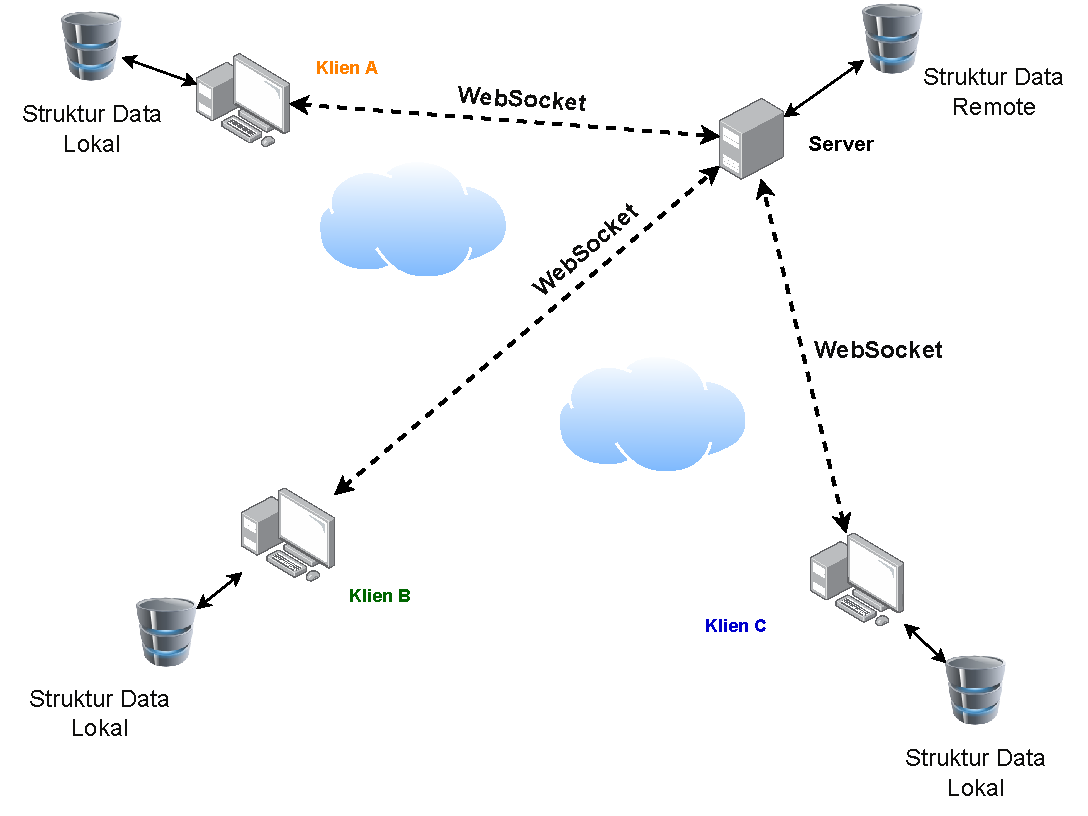
\includegraphics[scale=0.65]{assets/skripsi/Arsitektur_WebSocket_OT}
    \caption{Arsitektur yang Menggunakan WebSocket dan \textit{Operational Transformation}}
    \label{fig:websocket_ot}
\end{figure}

Untuk suatu dokumen yang hanya menyimpan teks biasa (\textit{plain text}), operasi \textit{operational transformation} yang hanya memenuhi sifat \textit{TP1} dapat diimplementasi dengan sederhana dalam arsitektur \textit{client-server}. Algoritma bekerja dengan menyimpan sebuah \textit{array} perubahan lokal yang belum diketahui oleh server. Perubahan-perubahan lokal beserta versi dokumen yang dapat disimpulkan dari banyaknya perubahan yang sudah dilakukan dari awal dokumen akan dikirimkan secara berkala dengan mekanisme RPC over WebSocket. Mekanisme ini pada dasarnya mengizinkan alur \textit{non-blocking} dalam menunggu balasan sebelum mengirimkan percobaan pengiriman perubahan lainnya. Apabila versi dasar dari server lebih baru daripada versi lokal, maka pengiriman perubahan akan ditolak, dan server akan memberikan respons kepada klien tersebut untuk melakukan \textit{rebase} atau menambahkan \textit{update} yang terdapat di server terlebih dahulu sebelum dapat mengirim percobaan pengiriman lagi.

Perubahan \textit{remote} yang diterima dari server akan ditransformasikan satu sama lain dengan perubahan lokal yang belum diketahui oleh server. Perubahan lokal akan ditimpa dengan perubahan yang sudah ditransformasikan dengan perubahan \textit{remote}. Percobaan pengiriman yang dikirim selanjutnya akan mengikuti perubahan yang sudah ditransformasikan ini. \textit{Operational transformation} hanya terjadi di lokal dan perubahan akan diperbarui secara seri, sehingga setiap dokumen dalam jaringan memiliki replika yang berujung identik dan konvergen.

Hal yang serupa diterapkan pula untuk \textit{shell} program yang berjalan. Saat suatu klien memberikan \textit{keystroke} pada salah satu \textit{shell} yang aktif, \textit{keystroke} akan dikirimkan melalui RPC yang serupa, namun akan diarahkan ke klien yang menjadi \textit{host} atau menjalankan programnya. Selanjutnya, perubahan \textit{shell} akan dikirimkan berkala pada server selama ada perubahan yang belum diterima atau diketahui server. Saat terjadi perubahan, server akan melakukan pengumuman untuk memberitahu kepada setiap klien untuk melakukan \textit{pull}. Karena respons \textit{shell} tergantung pada klien \textit{host}, maka pembaharuan tidak perlu diterapkan fungsi transformasi seperti pada OT teks biasa. Salah satu aspek lainnya ialah \textit{position mapping} yang tidak perlu ditangani karena kursor akan selalu berada di sebelah kanan karakter terakhir. Operasi seperti mekanisme \textit{update} yang dilaksanakan secara serial ini diterapkan untuk mencegah terjadinya \textit{race condition} pada saat gangguan jaringan.

\section{Desain Evaluasi}
\label{sec:desain_evaluasi}